\chapter{Specifikacija programske potpore}
		
	\section{Funkcionalni zahtjevi}
			
			
			

			
			\noindent \textbf{Dionici:}
			
			\begin{packed_enum}
				
				\item Poduzeće
				\item Ovlašteni distributeri ili 'leasing' kuće				
				\item Administrator baze podataka
				\item Razvojni tim
				
			\end{packed_enum}
			
			\noindent \textbf{Aktori i njihovi funkcionalni zahtjevi:}
			
			
			\begin{packed_enum}
				\item  \underbar{Gost - neprijavljeni korisnik (inicijator) ima sljedeće mogućnosti:}
				
				\begin{packed_enum}
					
					\item pregled raspoloživih vozila poduzeća
					\item pregled mjesta razmjene vozila
					\item pristup osnovnim kontaktima poduzeća
					\item izrada vlastitog korisničkog računa
					\item odabir vlasnika uz prikaz općih informacija o vlasniku
					\item prikaz recenzija i ocjena prodavača
					\item pregled vozila po kategoriji i vrsti
					\item pregled dostupnosti vozila
					
				\end{packed_enum}
				
					\item  \underbar{Korisnik - najmoprimac (inicijator) ima sljedeće mogućnosti:}
				
				\begin{packed_enum}
					
					\item promjena osobnih podataka uz naknadnu autorizaciju administratora
					\item pregled raspoloživih vozila poduzeća
					\item pregled mjesta razmjene vozila
					\item pristup osnovnim kontaktima poduzeća
					\item pregled kategorija po kategoriji i po vrsti
					\item odabir jednog od predloženih mjesta i vremena preuzimanja i isporuke vozila za unajmljivanja
					\item korištenje posebne usluge odabira vlastitog mjesta i vremena preuzimanja i isporuke za unajmljivanja
					\item uređivanje najmova
					\item brisanje vlastitog korisničkog računa
					\item pregled prethodnih najmova
					\item pisanje recenzija i dodjeljivanje ocjena
					
				\end{packed_enum}
				
					\item  \underbar{Administrator (inicijator) ima sljedeće mogućnosti:}
				
				\begin{packed_enum}
					
					\item pregled trenutno aktivnih prijavljenih korisnika
					\item pristup kontaktima pohranjenim u bazi podataka
					\item upis podataka o poduzećima
					\item autorizacija zatraženih promjena podataka računa
					\item brisanje korisničkih računa
					\item brisanje neprimjerenih recenzija
					\item određivanje vlasnika sustava
					
				\end{packed_enum}
				
					\item  \underbar{Vlasnik (inicijator) ima sljedeće mogućnosti:}
				
				\begin{packed_enum}
					
					\item pristup statistici poduzeća
					\item pregled svih vozila u voznom parku
					\item dodavanje novih vozila
					\item pristup i promjena podataka vozila
					\item dodavanje mjesta razmjene vozila
					\item brisanje mjesta razmjene vozila
					\item kategorizacija vozila
					
				\end{packed_enum}
			
				\item  \underbar{Baza podataka (sudionik) može:}
				
				\begin{packed_enum}
					
					\item pohrana podataka o vlasnicima i pripadnim vozilima
					\item pohrana podataka o korisnicima 
					
				\end{packed_enum}
			\end{packed_enum}
			
			\eject 
			
			
				
			\subsection{Obrasci uporabe}
				
				\textbf{\textit{Dio 1. revizije}}\\
					

					\noindent \underbar{\textbf{UC 1 - Registracija korisnika}}
					\begin{packed_item}
	
						\item \textbf{Glavni sudionik: }Gost
						\item  \textbf{Cilj: }Unijeti novog korisnika u sustav
						\item  \textbf{Sudionici: }Baza podataka
						\item  \textbf{Preduvjet: }-
						\item  \textbf{Opis osnovnog tijeka: }
						
						\item[] \begin{packed_enum}
							\item Gost ulazi u zaslon za registraciju
							\item Gost unosi sve potrebne podatke
							\item Gost je registriran i sada je korisnik
						\end{packed_enum}
						
						\item  \textbf{Opis mogućih odstupanja:}
						
						\item[] \begin{packed_item}
	
							\item[2.a] Uneseni podatci nisu u pravilnom formatu
							\item[] \begin{packed_enum}
								\item Aplikacija upozorava gosta i traži ga novi unos
							\end{packed_enum}
						\end{packed_item}
					\end{packed_item}
					
					\noindent \underbar{\textbf{UC 2 - Prijava korisnika}}
					\begin{packed_item}
	
						\item \textbf{Glavni sudionik: }Gost
						\item  \textbf{Cilj: }Prijaviti se u sustav
						\item  \textbf{Sudionici: }Baza podataka
						\item  \textbf{Preduvjet: }Korisnik je registriran u sustavu
						\item  \textbf{Opis osnovnog tijeka:}
						
						\item[] \begin{packed_enum}
							\item Uđi u zaslon za prijavu u sustav
							\item Unesi podatke za prijavu
						\end{packed_enum}
						
						\item  \textbf{Opis mogućih odstupanja:}
						
						\item[] \begin{packed_item}
	
							\item[2.a]  Uneseni podatci su netočni
							\item[] \begin{packed_enum}
								\item Aplikacija upozorava korisnika i traži ga novi unos i nudi mu odlazak na zaslon za registraciju
							\end{packed_enum}
						\end{packed_item}
					\end{packed_item}
					
					\noindent \underbar{\textbf{UC 3 - Pregled osobnih podataka}}
					\begin{packed_item}
	
						\item \textbf{Glavni sudionik: }Korisnik
						\item  \textbf{Cilj: }Dobiti uvid u vlastite podatke spremljene u sustavu
						\item  \textbf{Sudionici: }Baza podataka
						\item  \textbf{Preduvjet: }Korisnik je prijavljen u sustav
						\item  \textbf{Opis osnovnog tijeka:}
						
						\item[] \begin{packed_enum}
							\item Korisnik pristupa svojoj korisničkoj stranici i time ima uvid u svoje korisničke podatke
						\end{packed_enum}
						
						\item  \textbf{Opis mogućih odstupanja: }-
					\end{packed_item}
					
					\noindent \underbar{\textbf{UC 4 - Promjena osobnih podataka}}
					\begin{packed_item}
	
						\item \textbf{Glavni sudionik: }Korisnik
						\item  \textbf{Cilj: }Urediti vlastite korisničke podatke u sustavu
						\item  \textbf{Sudionici: }Baza podataka
						\item  \textbf{Preduvjet: }Korisnik je prijavljen u sustav
						\item  \textbf{Opis osnovnog tijeka:}
						
						\item[] \begin{packed_enum}
							\item Korisnik pristupa svojoj korisničkoj stranici
							\item Klikom na odgovarajući gumb otvara se sučelje u kojem korisnik ima mogućnost uređivanja podataka
						\end{packed_enum}
						
						\item  \textbf{Opis mogućih odstupanja:}
						
						\item[] \begin{packed_item}
	
							\item[2.a] Neki od unesenih podataka nije u pravilnom formatu
							\item[] \begin{packed_enum}
								\item Aplikacija upozorava korisnika i traži ga novi unos podatka
							\end{packed_enum}
						\end{packed_item}
					\end{packed_item}
					
					\noindent \underbar{\textbf{UC 5 - Pregled prijašnjih rezervacija}}
					\begin{packed_item}
	
						\item \textbf{Glavni sudionik: }Korisnik
						\item  \textbf{Cilj: }Dobiti uvid u sve prijašnje rezervacije vozila
						\item  \textbf{Sudionici: }Baza podataka
						\item  \textbf{Preduvjet: }Korisnik je prijavljen u sustav
						\item  \textbf{Opis osnovnog tijeka:}
						
						\item[] \begin{packed_enum}
							\item Korisnik pristupa svojoj korisničkoj stranici
							\item Klikom na odgovarajući gumb prikazuju se sve prijašnje korisnikove narudžbe
						\end{packed_enum}
						
						\item  \textbf{Opis mogućih odstupanja: }-
					\end{packed_item}
					
					\noindent \underbar{\textbf{UC 6 - Brisanje korisničkog računa}}
					\begin{packed_item}
	
						\item \textbf{Glavni sudionik: }Korisnik
						\item  \textbf{Cilj: }Ukloniti zapis o korisniku iz baze podataka
						\item  \textbf{Sudionici: }Baza podataka
						\item  \textbf{Preduvjet: }Korisnik je prijavljen u sustav
						\item  \textbf{Opis osnovnog tijeka:}
						
						\item[] \begin{packed_enum}
							\item Korisnik pristupa svojoj korisničkoj stranici
							\item Prilikom uređivanja računa ima priliku i izbrisati svoj račun
							\item Klikom na odgovarajuće dugme i potvrdom odabira briše se korisnički račun
						\end{packed_enum}
						
						\item  \textbf{Opis mogućih odstupanja: }-
					\end{packed_item}
					
					\noindent \underbar{\textbf{UC 7 - Pretraga vozila}}
					\begin{packed_item}
	
						\item \textbf{Glavni sudionik: }Gost, korisnik
						\item  \textbf{Cilj: }Pretražiti slobodna vozila po određenom kriteriju
						\item  \textbf{Sudionici: }Baza podataka
						\item  \textbf{Preduvjet: }-
						\item  \textbf{Opis osnovnog tijeka:}
						
						\item[] \begin{packed_enum}
							\item Korisnik bira datum i mjesto preuzimanja te vraćanja vozila. Za to su mu na raspolaganju kalendar i popis mogućih lokacija te karta
							\item Korisnik bira kategoriju vozila koje želi unajmiti
							\item Ispisuje se popis svih vozila koje odgovaraju korisnikovim kriterijima
							\item Klikom na za to predviđeno dugme traži se rezervacija vozila
						\end{packed_enum}
						
						\item  \textbf{Opis mogućih odstupanja: }
						
						\item[] \begin{packed_item}
	                        
	                        \item[1.a] Korisnik je odabrao vrijeme izvan besplatnog perioda (9.00 - 15.00)
							\item[] \begin{packed_enum}
								\item Za to korisnik plaća dodatnu naknadu
							\end{packed_enum}
							\item[1.b] Korisnik je izabrao mjesto drukčije od onog ponuđenog u popisu predefiniranih lokacija.
							\item[] \begin{packed_enum}
								\item Za to korisnik plaća dodatnu naknadu
							\end{packed_enum}
							\item[4.a] Gost nije prijavljen u sustav i traži rezervaciju
							\item[] \begin{packed_enum}
								\item Aplikacija ga preusmjerava na zaslon za prijavu i nakon prijave mu omogućuje rezervaciju
							\end{packed_enum}
						\end{packed_item}
						
					\end{packed_item}
					
					\noindent \underbar{\textbf{UC 8 - Rezervacija vozila}}
					\begin{packed_item}
	
						\item \textbf{Glavni sudionik: }Korisnik
						\item  \textbf{Cilj: }Rezervirati vozilo za iznajmljivanje
						\item  \textbf{Sudionici: }Baze podataka
						\item  \textbf{Preduvjet: }Korisnik je prijavljen u sustav i postoje slobodna vozila
						\item  \textbf{Opis osnovnog tijeka:}
						
						\item[] \begin{packed_enum}
							\item Korisnik pretražuje vozilo po prethodnom scenariju
							\item Klikom na željeno vozilo otvara se zaslon za plaćanje, na kojem korisnik plaća za rezervaciju zajedno s predujmom
							\item Rezervacija je napravljena i vidljiva je na korisničkim stranicama
						\end{packed_enum}
						
						\item  \textbf{Opis mogućih odstupanja: }-
					\end{packed_item}
					
					\noindent \underbar{\textbf{UC 9 - Promjena rezervacije}}
					\begin{packed_item}
	
						\item \textbf{Glavni sudionik: }Korisnik
						\item  \textbf{Cilj: }Urediti postojeću rezervaciju produljivanjem ili skraćivanjem perioda rezervacije
						\item  \textbf{Sudionici: }Baza podataka
						\item  \textbf{Preduvjet: }Postoji aktivna rezervacija i vozilo mora biti dostupno u novom željenom terminu
						\item  \textbf{Opis osnovnog tijeka:}
						
						\item[] \begin{packed_enum}
							\item Korisnik odlazi na popis svojih rezervacija.
							\item Klikom na odgovarajući gum ima opciju promijeniti datum preuzimanja (ako vozilo već nije preuzeto) i vraćanja vozila.
							\item Dodatni iznos za plaćanje koji je nastao razriješit će se prilikom povrata vozila.
						\end{packed_enum}
						
						\item  \textbf{Opis mogućih odstupanja: }
						
						\item[] \begin{packed_item}
	
							\item[2.a] Vozilo u novoodabranom terminu nije dostupno
							\item[] \begin{packed_enum}
								\item Aplikacija upozorava korisnika i ne dozvoljava mu postavljanje na taj datum.
							\end{packed_enum}
						\end{packed_item}
					\end{packed_item}
					
					\noindent \underbar{\textbf{UC 10 - Otkazivanje rezervacije}}
					\begin{packed_item}
	
						\item \textbf{Glavni sudionik: }Korisnik
						\item  \textbf{Cilj: }Otkazati napravljenu rezervaciju
						\item  \textbf{Sudionici: }Baza podataka
						\item  \textbf{Preduvjet: }Korisnik je prijavljen u sustav i postoji aktivna rezervacija, a vozilo još nije preuzeto
						\item  \textbf{Opis osnovnog tijeka:}
						
						\item[] \begin{packed_enum}
							\item Korisnik odlazi na popis aktivnih rezervacija.
							\item Iz popisa bira aktivnu rezervaciju koju želi otkazati
							\item Klikom na odgovarajući gumn korisnik briše rezervaciju
						\end{packed_enum}
						
						\item  \textbf{Opis mogućih odstupanja: }
						
						\item[] \begin{packed_item}
	
							\item[3.a] Do predviđenog vremena preuzimanja ostala su manje od 24 sata 
							\item[] \begin{packed_enum}
								\item Korisniku se naplaćuje određen iznos
							\end{packed_enum}
						\end{packed_item}
					\end{packed_item}
					
					\noindent \underbar{\textbf{UC 11 - Recenziranje usluge}}
					\begin{packed_item}
	
						\item \textbf{Glavni sudionik: }Korisnik
						\item  \textbf{Cilj: }Nakon povrata bozila ostaviti recenziju na uslugu
						\item  \textbf{Sudionici: }Baza podataka
						\item  \textbf{Preduvjet: }Korisnik je prijavljen, a usluga koja se ocjenjuje završila je
						\item  \textbf{Opis osnovnog tijeka:}
						
						\item[] \begin{packed_enum}
							\item Korisnik u popisu svojih prijašnjih rezervacija može recenzirati i mijenjati postojeće recenzije u rangu od jedne do pet zvjezdica
						\end{packed_enum}
						
						\item  \textbf{Opis mogućih odstupanja: }-
					\end{packed_item}
					
					\noindent \underbar{\textbf{UC 12 - Prikaz karte s navedenim poslovnicama}}
					\begin{packed_item}
	
						\item \textbf{Glavni sudionik: }Gost, korisnik, vlasnik sustava
						\item  \textbf{Cilj: }Na karti vidjeti prikazane sve poslovnice tvtrke za rent-a-car
						\item  \textbf{Sudionici: }Baza podataka
						\item  \textbf{Preduvjet: }-
						\item  \textbf{Opis osnovnog tijeka:}
						
						\item[] \begin{packed_enum}
							\item Prikaz karte bit će dostupan na naslovnoj stranici aplikacije te prilikom odabira mjesta preuzimanja i povrata vozila
							\item Na karti će biti označene poslovnice na koje će se moći kliknuti i vidjeti informacije o toj poslovnici, ili ju odabrati kao lokaciju preuzimanja i/ili povrata vozila
						\end{packed_enum}
						
						\item  \textbf{Opis mogućih odstupanja: }-
					\end{packed_item}
					
					\noindent \underbar{\textbf{UC 13 - Dodavanje vozila}}
					\begin{packed_item}
	
						\item \textbf{Glavni sudionik: }Vlasnik sustava
						\item  \textbf{Cilj: }Dodati novo vozilo u bazu podataka
						\item  \textbf{Sudionici: }Baza podataka
						\item  \textbf{Preduvjet: }Vlasnik je prijavljen u usustav
						\item  \textbf{Opis osnovnog tijeka:}
						
						\item[] \begin{packed_enum}
							\item U sučelju određenom za uređivanje popisa vozila vlasnik ima opciju dodavanja novog vozila
							\item Vlasnik unosi sve potrebne informacije o vozilu; slike, tehničke specifikacije, kategoriju i slično.
							\item Vozilo je sada vidljivo korisnicima i spremno za iznajmljivanje
						\end{packed_enum}
						
						\item  \textbf{Opis mogućih odstupanja: }
						
						\item[] \begin{packed_item}
	
							\item[2.a] Neki od unesenih podataka nisu u pravilnom formatu
							\item[] \begin{packed_enum}
								\item Aplikacija upozorava vlasnika i traži ga točan unos
							\end{packed_enum}
						\end{packed_item}
					\end{packed_item}
					
					\noindent \underbar{\textbf{UC 14 - Uklanjanje vozila}}
					\begin{packed_item}
	
						\item \textbf{Glavni sudionik: }Vlasnik sustava
						\item  \textbf{Cilj: }Neko vozilo ukloniti iz baze podataka
						\item  \textbf{Sudionici: }Baza podataka
						\item  \textbf{Preduvjet: }Vlasnik je prijavljen u usustav
						\item  \textbf{Opis osnovnog tijeka:}
						
						\item[] \begin{packed_enum}
							\item U sučelju određenom za uređivanje popisa vozila vlasnik ima opciju uklanjanja vozila
							\item Klikom na za to predviđeno digme i potvrdom vozilo će se ukloniti iz baze
							\item Vozilo više nije vidljivo korisnicima i ne može se unajmiti. 
						\end{packed_enum}
						
						\item  \textbf{Opis mogućih odstupanja: }-
					\end{packed_item}
					
					\noindent \underbar{\textbf{UC 15 - Uređivanje podataka o vozilu}}
					\begin{packed_item}
	
						\item \textbf{Glavni sudionik: }Vlasnik sustava
						\item  \textbf{Cilj: }Urediti određene informacije o vozilu
						\item  \textbf{Sudionici: }Baza podataka
						\item  \textbf{Preduvjet: }Vlasnik je prijavljen u usustav
						\item  \textbf{Opis osnovnog tijeka:}
						
						\item[] \begin{packed_enum}
							\item U sučelju određenom za uređivanje popisa vozila vlasnik ima opciju uređivanja informacija o vozilu
							\item Vlasnik mijenja podatke o vozilu
							\item Promjene su sada vidljive korisnicima 
						\end{packed_enum}
						
						\item  \textbf{Opis mogućih odstupanja: }
						
						\item[] \begin{packed_item}
	
							\item[2.a] Neki od unesenih podataka nisu u pravilnom formatu
							\item[] \begin{packed_enum}
								\item Aplikacija upozorava vlasnika i traži ga točan unos
							\end{packed_enum}
						\end{packed_item}
					\end{packed_item}
					
					\noindent \underbar{\textbf{UC 16 - Prikaz profitabilnosti i prijašnjih narudžbi}}
					\begin{packed_item}
	
						\item \textbf{Glavni sudionik: }Vlasnik sustava
						\item  \textbf{Cilj: }Dobiti uvid u sve prijašnje narudžbe i prikaz profitabilnosti procesa
						\item  \textbf{Sudionici: }Baza podataka
						\item  \textbf{Preduvjet: }Vlasnik je prijavljen u sustav
						\item  \textbf{Opis osnovnog tijeka:}
						
						\item[] \begin{packed_enum}
							\item U sučelju određenom za praćenje narudžbi vlasnik ima opciju pregledati povijest svih dosadašnjih narudžbi
							\item Vlasnik bira za koji vremenski period želi pregledati narudžbe, npr. all-time, prošlu godinu, prošli mjesec, prosinac 2018. i slično.
							\item Povijest se prikazuje u obliku popisa ili grafički, ovisno kako to korisnik odabere
						\end{packed_enum}
						
						\item  \textbf{Opis mogućih odstupanja:}
						
						\item[] \begin{packed_item}
	
							\item[2.a] Ne postoje narudžbe u odabranom vremenskom periodu
							\item[] \begin{packed_enum}
								\item Umjesto popisa se ispisuje prikladna poruka
							\end{packed_enum}
						\end{packed_item}
					\end{packed_item}
					
					\noindent \underbar{\textbf{UC 17 - Prikaz slobodnih vozila}}
					\begin{packed_item}
	
						\item \textbf{Glavni sudionik: }Vlasnik sustava
						\item  \textbf{Cilj: }Dobiti uvid u popis trenutno slobodnih vozila
						\item  \textbf{Sudionici: }Baza podataka
						\item  \textbf{Preduvjet: }Vlasnik je prijavljen u sustav
						\item  \textbf{Opis osnovnog tijeka:}
						
						\item[] \begin{packed_enum}
							\item U sučelju određenom za praćenje narudžbi vlasnik ima opciju pregledati sva trenutno slobodna vozila
						\end{packed_enum}
						
						\item  \textbf{Opis mogućih odstupanja:}
						
						\item[] \begin{packed_item}
	
							\item[1.a] Ne postoje slobodna vozila
							\item[] \begin{packed_enum}
								\item Umjesto popisa se ispisuje prikladna poruka
							\end{packed_enum}
						\end{packed_item}
					\end{packed_item}
					
					\noindent \underbar{\textbf{UC 18 - Prikaz aktivnih rezervacija}}
					\begin{packed_item}
	
						\item \textbf{Glavni sudionik: }Vlasnik sustava
						\item  \textbf{Cilj: }Dobiti uvid u popis trenutno zauzetih vozila
						\item  \textbf{Sudionici: }Baza podataka
						\item  \textbf{Preduvjet: }Vlasnik je prijavljen u sustav
						\item  \textbf{Opis osnovnog tijeka:}
						
						\item[] \begin{packed_enum}
							\item U sučelju određenom za praćenje narudžbi vlasnik ima opciju pregledati sva trenutno zauzeta vozila
							\item Prikazuju se osnovne info o zauzetom vozilu, npr. ime korisnika koji trenutno koristi uslugu, predviđeno vrijeme vraćanja i sl.
						\end{packed_enum}
						
						\item  \textbf{Opis mogućih odstupanja:}
						
						\item[] \begin{packed_item}
	
							\item[2.a] Ne postoje zauzeta vozila
							\item[] \begin{packed_enum}
								\item Umjesto popisa se ispisuje prikladna poruka
							\end{packed_enum}
						\end{packed_item}
					\end{packed_item}
					
					\noindent \underbar{\textbf{UC 19 - Zatvaranje rezervacije}}
					\begin{packed_item}
	
						\item \textbf{Glavni sudionik: }Vlasnik vozila
						\item  \textbf{Cilj: }Rezervaciju označiti gotovom
						\item  \textbf{Sudionici: }Baza podataka
						\item  \textbf{Preduvjet: }Vlasnik je prijavljen u sustav, rezervacija je trenutno aktivna
						\item  \textbf{Opis osnovnog tijeka:}
						
						\item[] \begin{packed_enum}
							\item Po povratu vozila vlasnik sustava vrši pregled vozila kako bi se utvrdila možebitna oštećenja na vozilu
							\item Vlasnik izdaje pisanu potvrdu o završetku rezervacije i korisnik i vlasnik se novčano razdužuju
							\item Vlasnik rezervaciju označava završenom i vozilo je ponovo dostupno za iznajmljivanje drugim korisnicima
							\item Narudžba je sada vidljiva u popisu prošlih narudžbi
							\item Korisnik potvrdu vidi u svojim prijašnjim narudžbama
						\end{packed_enum}
						
						\item  \textbf{Opis mogućih odstupanja:} -
					\end{packed_item}
					
					
					\noindent \underbar{\textbf{UC 20 - Pregled korisnika}}
					\begin{packed_item}
	
						\item \textbf{Glavni sudionik: }Administrator
						\item  \textbf{Cilj: }Dobiti uvid u popis korisnika u bazi
						\item  \textbf{Sudionici: }Baza podataka
						\item  \textbf{Preduvjet: }Korisnik ima administratrorska prava
						\item  \textbf{Opis osnovnog tijeka:}
						
						\item[] \begin{packed_enum}
							\item Administrator ima uvid u popis svih korisnika prijavljenih u bazu
							\item Klikom na određenog korisnika iz popisa administrator ima uvid u sve podatke o njemu koji su u bazi zapisani
						\end{packed_enum}
						
						\item  \textbf{Opis mogućih odstupanja: }-
					\end{packed_item}
					
					\noindent \underbar{\textbf{UC 21 - Brisanje korisnika}}
					\begin{packed_item}
	
						\item \textbf{Glavni sudionik: }Administrator
						\item  \textbf{Cilj: }Određenog korisnika izbrisati iz baze
						\item  \textbf{Sudionici: }Baza podataka
						\item  \textbf{Preduvjet: }Korisnik ima administratorska prava
						\item  \textbf{Opis osnovnog tijeka:}
						
						\item[] \begin{packed_enum}
							\item Administrator ima uvid u popis svih korisnika prijavljenih u bazu
							\item Klikom na određenog korisnika administrator ima uvid u njega
							\item Klikom na odgovarajući gumn i potvrdom administrator briše korisnika
						\end{packed_enum}
						
						\item  \textbf{Opis mogućih odstupanja:}
						
						\item[] \begin{packed_item}
	
							\item[3.a] Administrator pokušava izbrisati samog sebe 
							\item[] \begin{packed_enum}
								\item Aplikacija mu to ne dozvoljava i javlja mu poruku
							\end{packed_enum}
						\end{packed_item}
					\end{packed_item}
					
					\noindent \underbar{\textbf{UC 22 - Promjena razine korisnika}}
					\begin{packed_item}
	
						\item \textbf{Glavni sudionik: }Administrator
						\item  \textbf{Cilj: }Za određenog korisnika promijeniti razinu prava
						\item  \textbf{Sudionici: }Baza podataka
						\item  \textbf{Preduvjet: }Korisnik ima administratorska prava
						\item  \textbf{Opis osnovnog tijeka:}
						
						\item[] \begin{packed_enum}
							\item Administrator ima uvid u popis svih korisnika prijavljenih u sustav
							\item Klikom na odrešenog korisnika administrator ima uvid u njega
							\item Administrator može promijeniti razinu korisnika, iz običnog u vlasnika sustava i obrnuto
						\end{packed_enum}
						
						\item  \textbf{Opis mogućih odstupanja:}
						
						\item[] \begin{packed_item}
	
							\item[2.a] Administrator pokušava promijeniti svoja prava iz administratorskih prava u neko niže
							\item[] \begin{packed_enum}
								\item Aplikacija mu to ne dozvoljava i javlja mu poruku
							\end{packed_enum}
						\end{packed_item}
					\end{packed_item}
					
					\noindent \underbar{\textbf{UC 23 - Dodavanje poslovnice}}
					\begin{packed_item}
	
						\item \textbf{Glavni sudionik: }Administrator
						\item  \textbf{Cilj: }Dodati novu poslovnicu u bazu podataka
						\item  \textbf{Sudionici: }Baza podataka
						\item  \textbf{Preduvjet: }Korisnik ima administratorska prava
						\item  \textbf{Opis osnovnog tijeka:}
						
						\item[] \begin{packed_enum}
							\item Administrator u sučelju ima mogućnost pregleda popisa svih poslovnica tvrtke
							\item Klikom na odgovarajuće dugme može dodati novu poslovicu
							\item Administrator dodaje sve potrebne informacije o poslovnici; Adresa, kontakt broj i sl.
							\item Ta je poslovnica vidljiva svim korisnicima u aplikaciji
						\end{packed_enum}
						
						\item  \textbf{Opis mogućih odstupanja: }
						
						\item[] \begin{packed_item}
	
							\item[3.a] Neki od unesenih podataka nisu u pravilnom formatu
							\item[] \begin{packed_enum}
								\item Aplikacija upozorava administratora i traži ga novi unos
							\end{packed_enum}
						\end{packed_item}
						
					\end{packed_item}
					
					\noindent \underbar{\textbf{UC 24 - Uklanjanje poslovnice}}
					\begin{packed_item}
	
						\item \textbf{Glavni sudionik: }Administrator
						\item  \textbf{Cilj: }Ukloniti poslovnicu iz baze podataka
						\item  \textbf{Sudionici: }Baza podataka
						\item  \textbf{Preduvjet: }Korisnik ima administratorska prava i postoje unesene poslovnice
						\item  \textbf{Opis osnovnog tijeka:}
						
						\item[] \begin{packed_enum}
							\item Administrator u sučelju ima mogućnost pregleda popisa svih poslovnica tvrtke
							\item Klikom na odgovarajuće dugme i potvrdom administrator uklanja poslovnicu
							\item Poslovnica više nije vidljiva korisnicima u aplikaciji
						\end{packed_enum}
						
						\item  \textbf{Opis mogućih odstupanja: }-
					\end{packed_item}
					
					\noindent \underbar{\textbf{UC 25 - Uređivanje poslovnice}}
					\begin{packed_item}
	
						\item \textbf{Glavni sudionik: }Administrator
						\item  \textbf{Cilj: }Urediti podatke o poslovnici
						\item  \textbf{Sudionici: }Baza podataka
						\item  \textbf{Preduvjet: }Korisnik ima administratorska prava i postoje unesene poslovnice
						\item  \textbf{Opis osnovnog tijeka:}
						
						\item[] \begin{packed_enum}
							\item Administrator u sučelju ima mogućnost pregleda popisa svih poslovnica tvrtke
							\item Klikom na određeno dugme administrator pristupa sučelju za uređivanje podataka o poslovnici
							\item Administrator unosi nove podatke i snima promjene
							\item Promjene su vidljive korisnicima u aplikaciji
						\end{packed_enum}
						
						\item  \textbf{Opis mogućih odstupanja: }
						
						\item[] \begin{packed_item}
	
							\item[3.a] Neki od unesenih podataka nisu u pravilnom formatu
							\item[] \begin{packed_enum}
								\item Aplikacija upozorava administratora i traži ga novi unos
							\end{packed_enum}
						\end{packed_item}
						
					\end{packed_item}
				
				\eject
				\subsubsection{Dijagrami obrazaca uporabe}
					
					\textit{Prikazati odnos aktora i obrazaca uporabe odgovarajućim UML dijagramom. Nije nužno nacrtati sve na jednom dijagramu. Modelirati po razinama apstrakcije i skupovima srodnih funkcionalnosti.}
						
				
				\begin{figure}[htb]
                    \centering
                    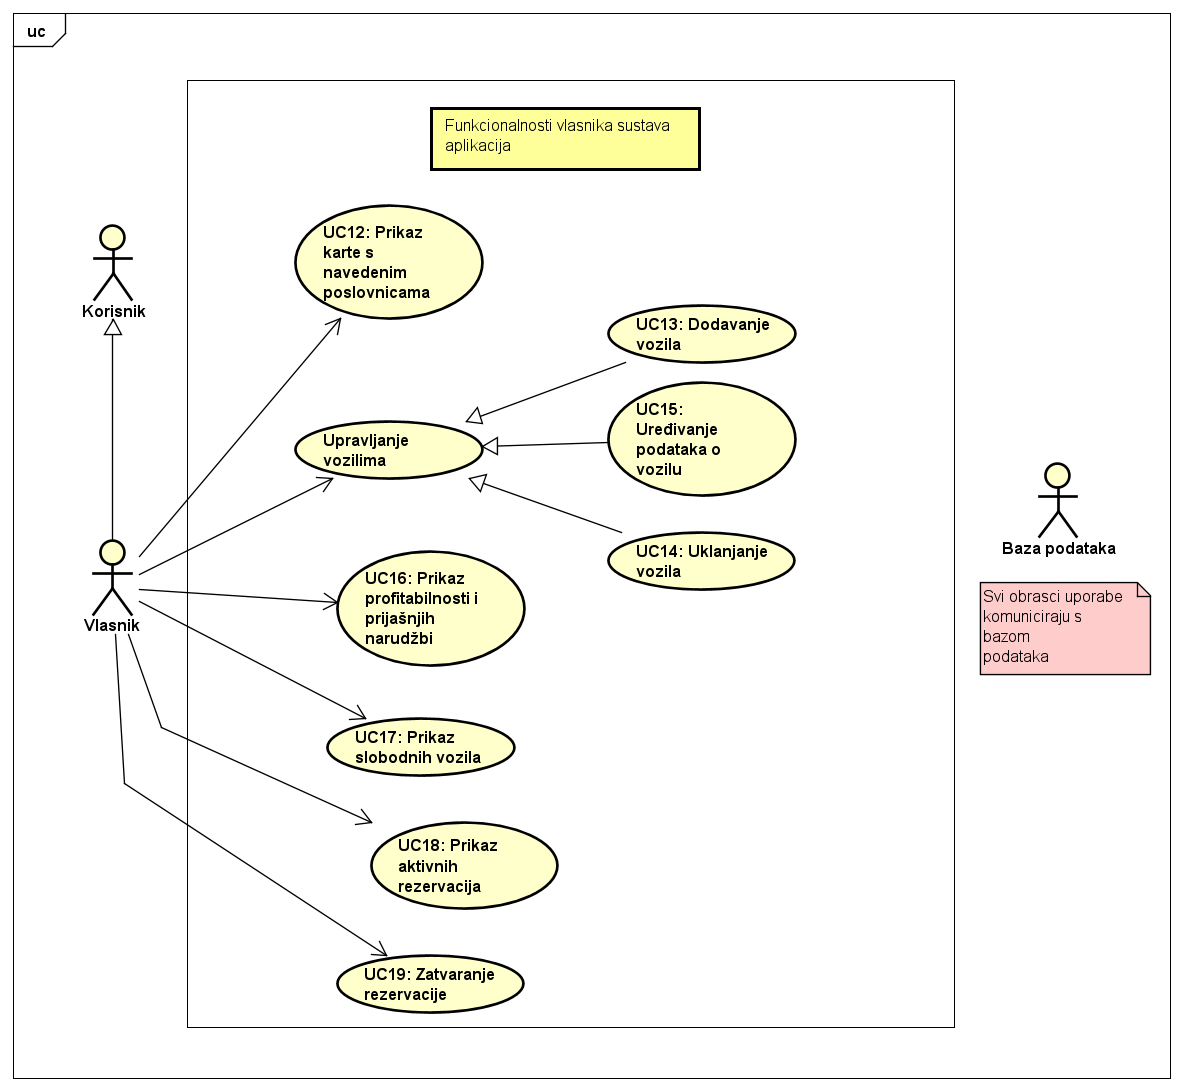
\includegraphics[width=15cm]{dokumentacija/slike/UseCaseDiagram1.png}
                    \caption{Dijagram obrasca uporabe, funkcionalnost vlasnika sustava}
                    \label{fig:useCase-1}
                \end{figure}
                \begin{figure}[htb]
                    \centering
                    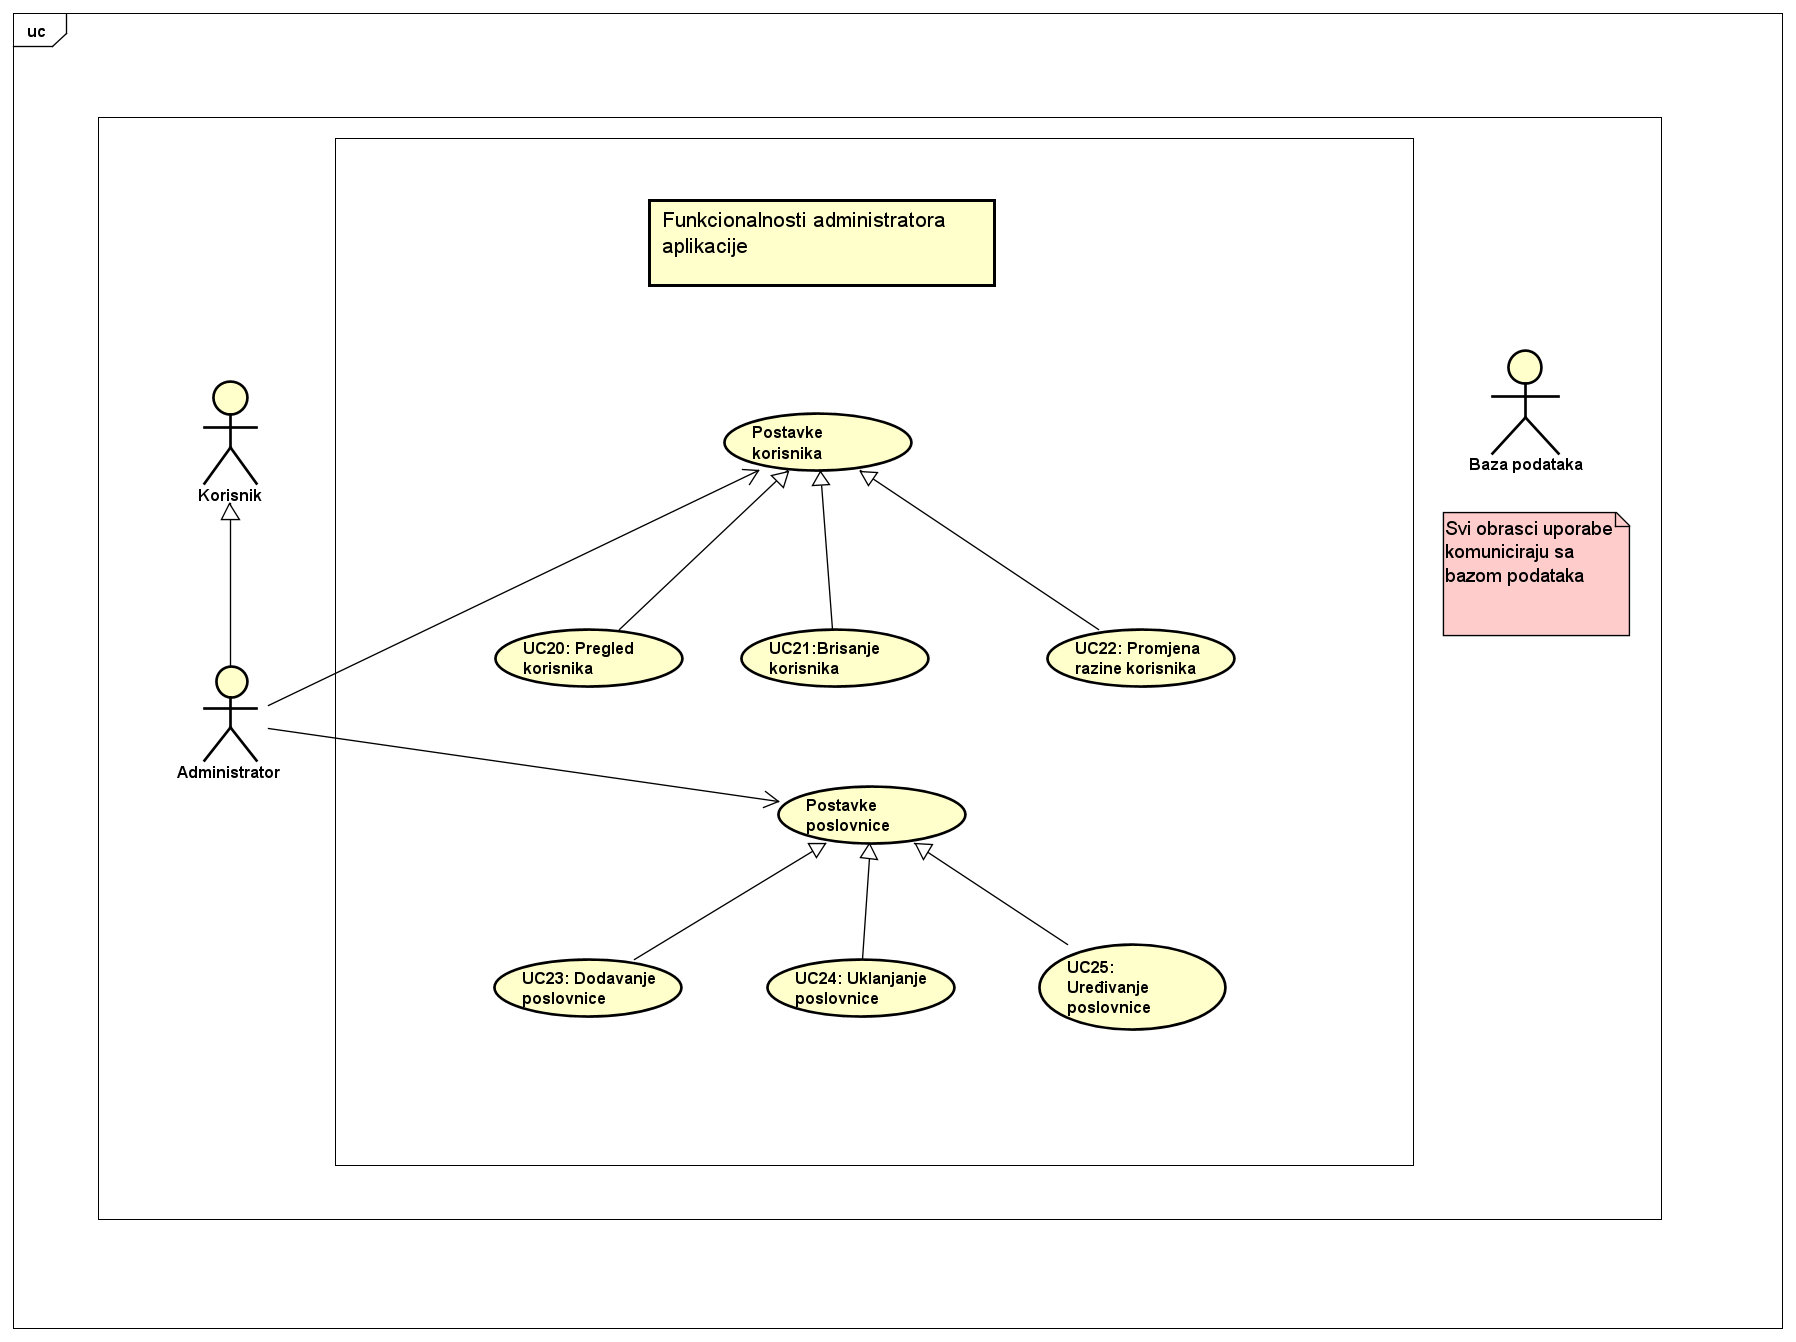
\includegraphics[width=15cm]{dokumentacija/slike/UseCaseDiagram2.png}
                    \caption{Dijagram obrasca uporabe, funkcionalnost administratora sustava}
                    \label{fig:useCase-2}
                \end{figure}
                
                
                \eject
				
			\subsection{Sekvencijski dijagrami}
				
				\textbf{\textit{dio 1. revizije}}\\
				
				\textit{Nacrtati sekvencijske dijagrame koji modeliraju najvažnije dijelove sustava (max. 4 dijagrama). Ukoliko postoji nedoumica oko odabira, razjasniti s asistentom. Uz svaki dijagram napisati detaljni opis dijagrama.}
				\eject
				
	
		\section{Nefunkcionalni zahtjevi}
		
		    	\textbf{\textit{Zahtjevi kvalitete:}}\\
		 
		\begin{packed_item}
	
						\item Sustav bi trebao jamčiti točnost i pouzdanost informacija.
						\item  Unos neispravnih oblika podataka ili upload krivih datoteka ne smije narušiti sustav.
						\item Odgovor na svaki upit ili zahtjev za nekom radnjom nebi trebao trajati duže od 1 sekunde.
						\item  Dizajn sustava mora omogućiti intuitivnu uporabu sustava.
						\item Sustav se mora moći nadograditi prema zahtjevima naručitelja
						
					\end{packed_item}
				
			 
	    	\textbf{\textit{Ograničenja:}}\\
		 
			\begin{packed_item}
	
						\item Programska podrška je izvedena kao Springboot web aplikacija pisana u Javi.
						\item  Pohrana podataka je izvedena preko Postgre SQL baze podataka.
						\item Programska podrška mora bit sposobna na CRUD operacije svih priloženih podataka.
						\item  Jedan korisnik ne može biti ulogiran na dva različita računala(istovremeno imati dvije aktivne sjednice)
						
					\end{packed_item}
			 
			 
			 
	